\chapter{Analiza danych pochodzących z serwisu Lending Club}

\section{Opis platformy Lending Club}

Lending Club to amerykański startup finansowy utworzony w 2006 z główną siedzibą znajdującą się w San Francisco, w stanie Kalifornia. Firma jest dostawcą platformy oferującej pożyczki w formacie \textit{peer-to-peer} - pożyczkobiorcy mogą pozyskiwać finansowanie bezpośrednio u potencjalnych pożyczkodawców, bez udziału instytucji postronnych \cite{LendingClub}. Jest to pierwsza spółka tego sektora, która zarejstrowała swoje produkty w amerykańskiej komisji papierów wartościowych (ang. \textit{US Securities and Exchange Comission}). Wszystkie operacje prowadzone są w ramach platformy internetowej, co pozwoliło na znaczną redukcję kosztów z jakimi muszą mierzyć się tradycyjne instytucje finansowe (np. koszty związane z utrzymywaniem placówek). Dzięki temu stopy procentowe przypisane do pożyczek są atrakcyjne zarówno dla kredytobiorców, jak i potencjalnych inwestorów. 

\subsection{Model biznesowy}

Założeniem Lending Club jest dostarczenie użytkownikom platformy, która umożliwi interakcję dwóm komplementarnym grupom - pożyczkobiorcom i inwestorom. Pożyczkobiorcy zgłaszają zapotrzebowanie na kredyt za pośrednictwem publicznie dostępnej listy pożyczek, przy czym kwota kredytu musi mieścić się w zakresie \$1000 - \$40000 a termin spłaty pożyczki musi wynosić 36 lub 60 miesięcy. Na podstawie danych użytkownia, zawierających informacje na temat jego historii kredytowej, bieżącej zdolności kredytowej, kwoty pożyczki o jaką się ubiega oraz jego stosunku zadłużenia do dochodu, pożyczce nadawany jest stopień z zakresu A-G (przy czym pożyczki oznaczone symbolem ``A'' oznaczają najniższy stopień ryzyka, a ``G'' najwyższy) oraz wyznaczana jest wysokość opłat i stopa zwrotu przypisana pożyczce \cite{LendingClub}. 

Inwestorzy mogą budować swoje portfolio ręcznie, wybierając pożyczki z dostępnej listy i określając kwotę inwestycj, lub korzystając z algorytmu automatycznie dobierającego zrównoważony portfel pożyczek. W przypadku podejmowania decyzji inwestycyjnych bezpośrednio przez inwestorów wzrasta znaczenie zewnętrznych systemów wspomagających podejmowanie decyzji. Taką rolę będzie pełnił system opracowany w ramach tej pracy magisterskiej - aplikacja będzie udostępniała użytkownikom statystyki wygenerowane na podstawie danych historycznych oraz moduł wyliczający prawdopodobieństwo niespłącenia pożyczki przez pożyczkobiorcę. W oparciu o te informacje dużo łatwiej jest zarządzać strategią inwestycyjną, polegającą na wczesnej sprzedaży pożyczek o zbyt wysokim ryzyku oraz skupowaniu pożyczek (dzięki predykcji z zastosowaniem algorytmów uczenia maszynowego, można określić to prawdopodobieństwo przed spadkiem wartości długu), które prawdopodobnie zostaną spłacone w terminie.

\section{Analiza udostępnionych danych}

Lending Club co kwartał publikuje dane opisujące pożyczki zawarte w poprzednim okresie rozliczeniowym wraz ze słownikiem opisującym te dane, który został załączony do tej pracy. Najpierw dokonano wstępnego przetworzenia danych, polegającego na:

\begin{itemize}
\item scaleniu danych z poszczególnych okresów w jeden plik
\item konwersji danych zawartych w następujących kolumnach do wartości numerycznych:
	\begin{itemize}
		\item int\_rate - stopa procentowa,
		\item revol\_util - procentowy skaźnik zużycia lini kredytowej,
		\item emp\_legth - długość zatrudnienia,
		\item term - okres spłaty pożyczki,
		\item pymnt\_plan - pożyczki, które mają rozpisany plan płatności zostały oznaczone wartością ``1'', w przeciwnym wypadku ``0''.
	\end{itemize}
\end{itemize}

Ponadto utworzono dodatkową kolumnę \textit{``defaulted''}, w której pożyczki uznane za niespłacone, tj. o statusie należącym do grupy: \textit{Charged Off, Default, Late (16-30 days), Late (31-120 days)}, zostały oznaczone wartością ``1'', a pozostałe wartością ``0''.

\subsection{Statystyki według stanu}

Bardzo istotną informacją z punktu widzenia inwestora jest popularność platformy w poszczególnych stanach. Na podstawie informacji na temat liczby pożyczek i łącznej kwoty, na którą zostały udzielone w poszczególnych stanach możliwe jest określenie potencjalnej liczby inwestorów i dynamikę rynku kredytowego w danym regionie. Dzięki tym danym inwestor jest świadomy, w jakim stopniu będzie mógł zarządzać długiem w przyszłości, np. czy łatwo będzie mu odsprzedać zadłużenie innemu inwestorowi. Kod generujący te statystyki został przedstawiony na Wydruku \ref{r:valueState} i \ref{r:volumeState}.

\begin{lstlisting}[language=R, caption={Skrypt wyliczający łączną kwotę udzielonych kredytów dla każdego stanu}, label={r:valueState}]
state_by_value <- loanbook %>% group_by(region) %>% 
	summarise(value = sum(loan_amnt, na.rm=TRUE))

state_choropleth(state_by_value, title = "Value by State")
\end{lstlisting}

\begin{figure}[h] \centering %H if want to get it exaclty here
	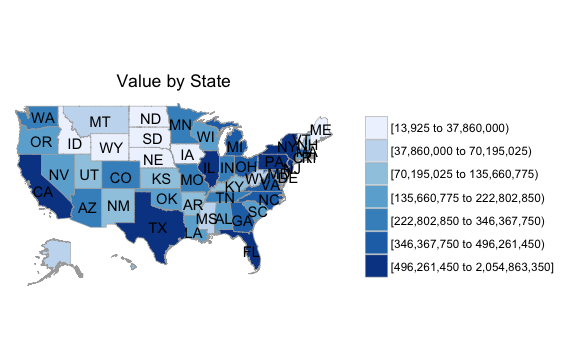
\includegraphics[scale=0.7]{img/value_state.png}
	\caption{Łączna kwota udzielonych kredytów wg. stanu.}
	\label{lc:value_state}
\end{figure}

Zarówno w przypadku liczby jak i łącznej kwoty udzielonych kredytów stanem o najwyższych statystykach jest Kalifornia. Wynika to przede wszystkim z zamożności społeczeństwa, ale również z faktu, że wiele firm technologicznych, w tym Lending Club, pochodzi właśnie z tego stanu i jest to rynek, na którym operują najdłużej i któremy poświęciły bardzo dużo uwagi. Usługi oferowane przez Lending Club cieszą się dużą popularnością w bogatych stanach, takich jak wspomniana Kalifornia, Teksas oraz stany wschodniego wybrzeża USA. Zdecydowanie mniej popularne są w uboższym rejonie północnych stanów USA. 

\begin{lstlisting}[language=R, caption={Skrypt wyliczający liczbę udzielonych kredytów dla każdego stanu}, label={r:volumeState}]
state_by_volume <- loanbook %>% group_by(region) %>%
  summarise(value = n())

state_choropleth(state_by_volume, title = "Volume by State")
\end{lstlisting}

\begin{figure}[h] \centering %H if want to get it exaclty here
	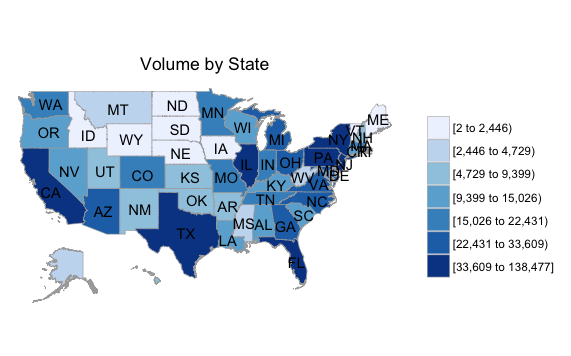
\includegraphics[scale=0.7]{img/volume_state.png}
	\caption{Liczba udzielonych kredytów wg. stanu.}
	\label{lc:volume_state}
\end{figure}

\subsection{Wysokość pożyczek}

Po zbadaniu rozkładu danych względem wysokości pożyczki (Rysunek \ref{lc:amnt_distrib}) okazało się, że mediana dla tych danych wynosi \$13225,00 a średnia wysokość \$14900,25. Obie te wartości są znacznie poniżej maksymalnego limitu wynoszącego \$40000 - ponadto 70\% wszystkich kredytów zostało udzielonych na kwotę nie większą niż \$20000, co stanowi połowę dopuszczalnego limitu.

\begin{figure}[h] \centering %H if want to get it exaclty here
	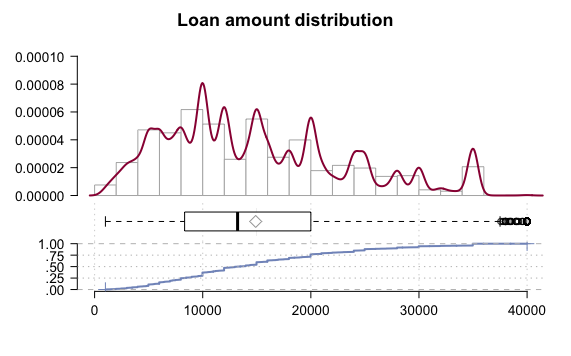
\includegraphics[scale=0.5]{img/loan_amt_distrib.png}
	\caption{Rozkład pożyczek względem ich wysokości.}
	\label{lc:amnt_distrib}
\end{figure}

Rysunek \ref{lc:amnt_growth} przedstawia wzrost ruchu na platformie na przestrzeni lat. Punktem przełomowym jest marzec 2014, kiedy firma weszła na giełdę - od tego czasu suma pożyczek zawartych na platformie uległa potrojeniu.

\begin{figure}[h] \centering %H if want to get it exaclty here
	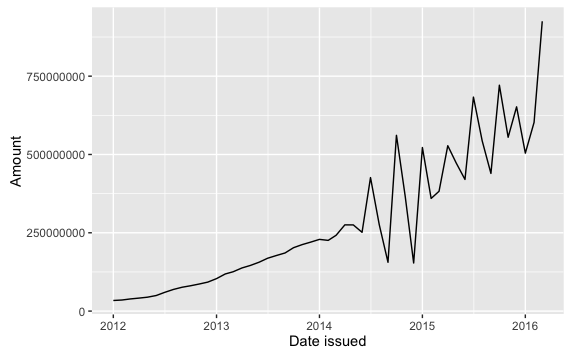
\includegraphics[scale=0.5]{img/loanbook_growth.png}
	\caption{Całkowita kwota pożyczek udzielonych w ramach Lending Club.}
	\label{lc:amnt_growth}
\end{figure}

\subsection{Powody zaciągania kredytów konsumenckich}

Wedlug serwisu Bankrate.com \cite{bankrate} najpopularniejsze powody zaciągania pożyczek konsumenckich w Stanach Zjednoczonych to:

\begin{itemize}
	\item konsolidacja długów,
	\item spłata kart kredytowych,
	\item remont domu,
	\item ślub,
	\item przeprowadzka,
	\item opłaty związane z pogrzebem bliskiej osoby,
	\item opłaty związane z leczeniem (w USA służba zdrowia nie ma charakteru publicznego),
	\item zakup samochodu,
	\item wakacje.
\end{itemize}

Znajduje to odzwieciedlenie w danych serwisu Lending Club (Rysunek \ref{lc:purposes}). Konsolidacja długów stanowi 59,5\% wszystkich zaciągniętych pożyczek, a druga pozycja w zestawieniu - spłata karty kredytowej - 23,8\%. Łącznie te dwie grupy stanowią ponad 80\% wszystkich kredytów. Jest to spowodowane nieustannym wzrostem zadłużenia społeczeństwa amerykańskiego - w 2015 roku całkowita kwota udzielonych kredytów konsumenckich wzrosła o 7\%, a w pierwszym kwartale 2016 o 5,8\% w stosunku do anologicznego okresu w ubiegłym roku \cite{federalreserve}.

\begin{figure}[h] \centering %H if want to get it exaclty here
	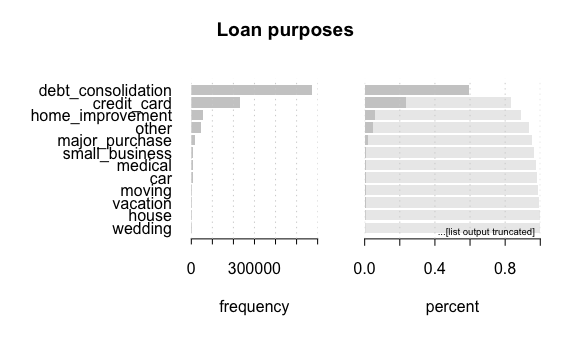
\includegraphics[scale=0.7]{img/purposes.png}
	\caption{Powody zaciągania pożyczek konsumenckich w Lending Club.}
	\label{lc:purposes}
\end{figure}

\subsection{Zdolność kredytowa użytkowników Lending Club}

Zdolność kredytowa użytkowników jest oceniana w siedmiostopniowej (Rysunek \ref{lc:grades}) skali na podstawie ich historii kredytowej oraz informacji o stanie zatrudnienia i posiadanych nieruchomościach. Najbezpieczniejsze pożyczki otrzymują kategorię A, natomiast te o największym stopniu ryzyka - G \cite{LendingClub}. Najliczniejszą grupę kredytów stanowią pożyczki o kategoriach B i C - w sumie stanowią prawie 60\% wszystkich pożyczek.

\begin{figure}[h] \centering %H if want to get it exaclty here
	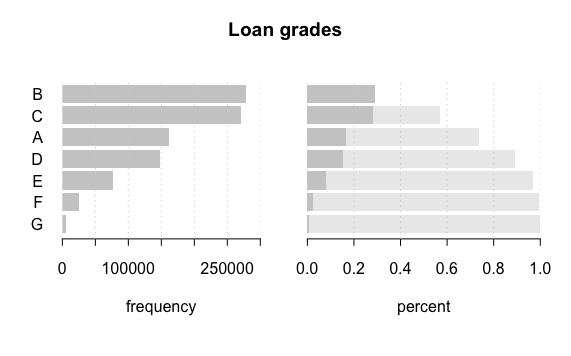
\includegraphics[scale=0.7]{img/grades.png}
	\caption{Kategorie pożyczek.}
	\label{lc:grades}
\end{figure}

Im większe ryzyko inwestycji, tym wyższysz zwrotów oczekują inwestorzy. Znajduje to odzwierciedlenie na wykresie przedstawiającym zależność wysokości stóp procentowych od kategorii pożyczki (Rysunek \ref{lc:int2grade}).

\begin{figure}[h] \centering %H if want to get it exaclty here
	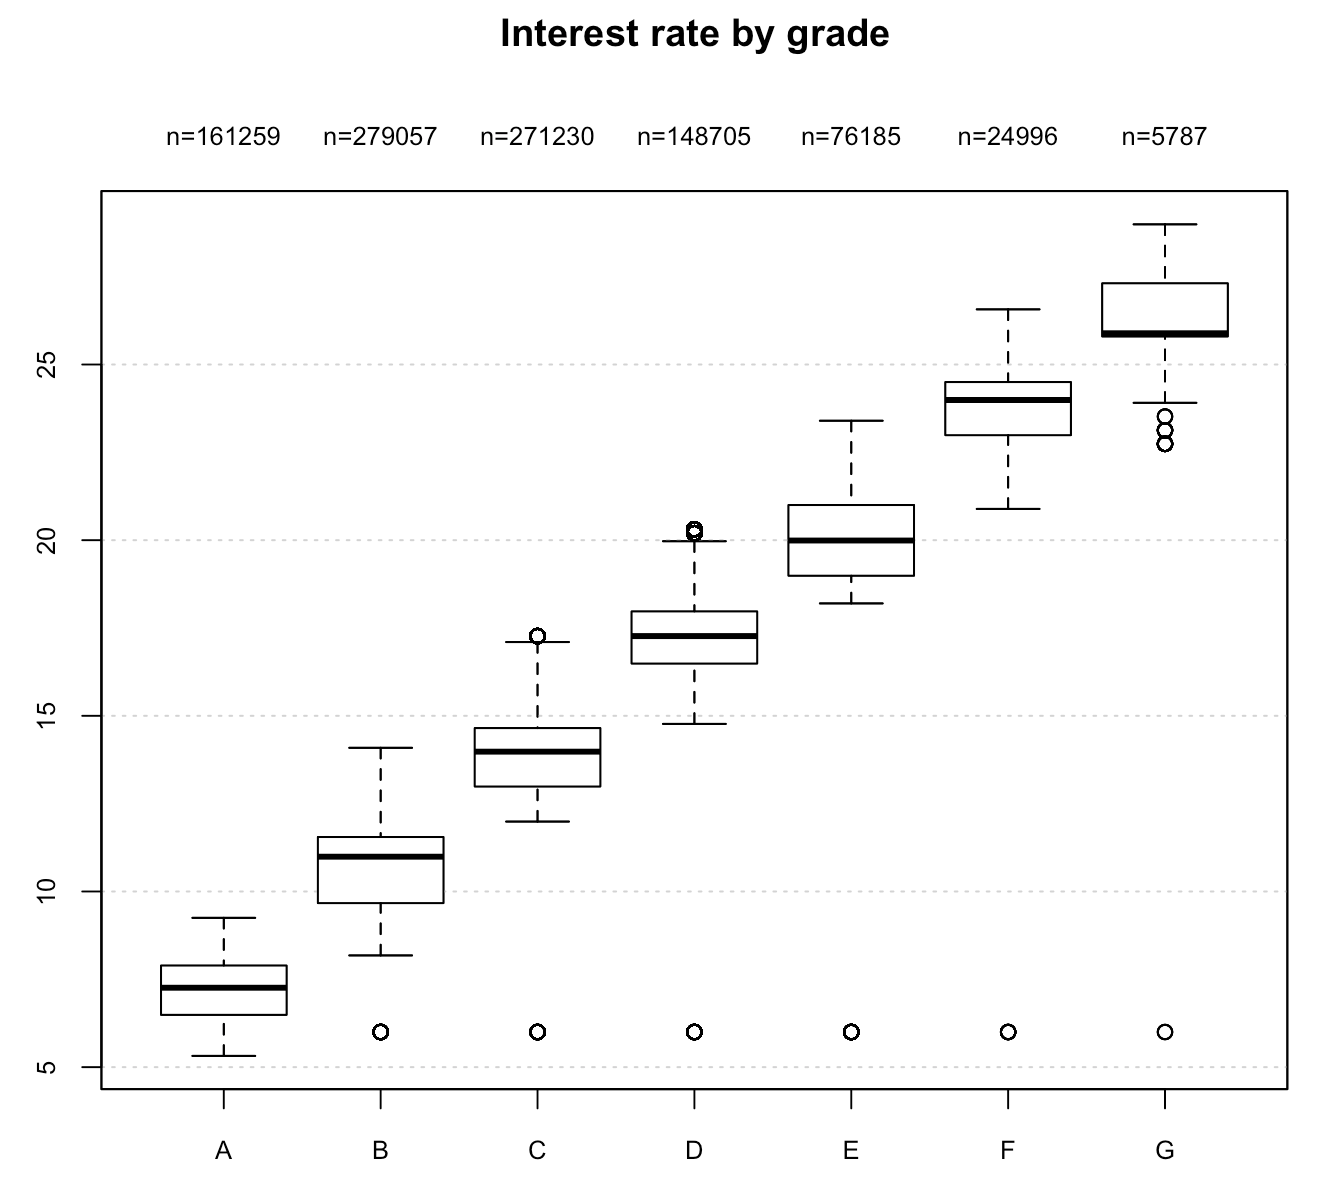
\includegraphics[scale=0.5]{img/int2grade.png}
	\caption{Zależność stóp procentowych od kategorii pożyczki.}
	\label{lc:int2grade}
\end{figure}

\subsection{Statusy pożyczek}

Każda z pożyczek ma przypisany status, który określa jej aktualny stan (Rysunek \ref{lc:statuses}). Najliczniejszymi grupami są bieżące pożyczki (\textit{Current}) i spłacone (\textit{Fully Paid}) - odpowiednio 66\% i 25,3\%, co stanowi 91,3\% wszystkich pozycji. Oznacza to, że 8,7\% pożyczek to pożyczki, które przyniosły straty inwestorom. Jednym z zadań implementowanego systemu będzie wyliczenie prawdopodobieństwa, że bieżąca pożyczka przestanie być spłacana w terminie lub w ogóle nie zostanie zpłacona. Inwestor dzięki tym informacjom będzie mógł aktywnie zarządzać swoim portfolio poprzez wczesną sprzedaż zadłużenia o zbyt dużym ryzyku oraz zakup długów o niskim prawdopodobieństwie niespłacalności. Wykorzystano do tego metodę regresji opartą na modelach uczenia maszynowego, co zostało opisane w następnym rozdziale. W celu przystosowania danych do przeprowadzenia regresji logistycznej, tj. przypadku gdy zmienna zależna przyjmuje tylko dwie wartości \cite{MED}, na etapie wstępnego przetwarzania danych utworzono dodatkową kolumnę \textbf{defaulted}, która przyjmuje wartości \textbf{0} dla pożyczek o pozytywnym lub neutralnym statusie (\textit{Current, Fully Paid, In Grace Period}) oraz \textbf{1} dla tych o negatywnym. Następnie przeprowadzono analizę zależności wartości nowoutworzonej kolumny od atrybutów numerycznych opisujących pożyczkę. Utworzono również dodatkowy atrybut opisujący procentowy stopień spłacenia długu.

\begin{figure}[h] \centering %H if want to get it exaclty here
	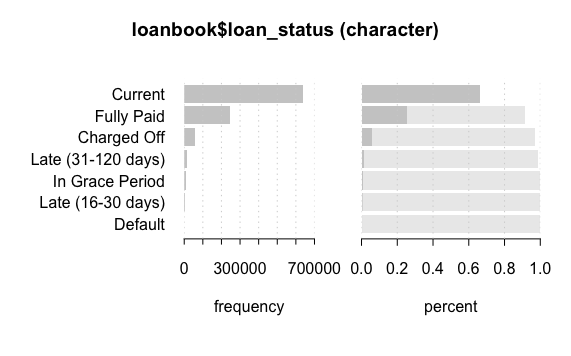
\includegraphics[scale=0.5]{img/statuses.png}
	\caption{Statusy pożyczek.}
	\label{lc:statuses}
\end{figure}

\subsection{Analiza wpływu zmiennych numerycznych na status pożyczki}

Ostatnim etapem analizy danych było zbadanie wpływy poszczególnych atrybutów numerycznych na zachowanie pożyczki. Wykorzystano w tym celu podział na \textit{dobre} i \textit{złe} pożyczki w oparciu o ich statu wprowadzone na etapie wstępnego przetwarzania (utworzenie kolumny \textbf{defaulted} przyjmującej wartości 0 i 1). 

\begin{lstlisting}[language=R, caption={Skrypt wyznaczający macierz koralacji dla zmiennych numerycznych.}, label={r:correlationMatrix}]
set.seed(123)
library(mlbench)
library(caret)

numeric_vars <- sapply(loanbook, is.numeric)
correlationMatrix <- cor(loanbook[, numeric_vars])
correlationMatrix[is.na(correlationMatrix)] <- 0
redundantData <- findCorrelation(correlationMatrix, cutoff = 0.9, verbose = TRUE, names = TRUE, exact = TRUE)
print(correlationMatrix[redundantData, redundantData])
\end{lstlisting}

W celu ograniczenia liczby badanych atrybutów wyznaczono macierz korelacji i usunięto ze zbioru te atrybuty, dla których współczynnik wyniósł ponad 90\% \ref{r:correlationMatrix}.

\begin{figure}[h] \centering %H if want to get it exaclty here
	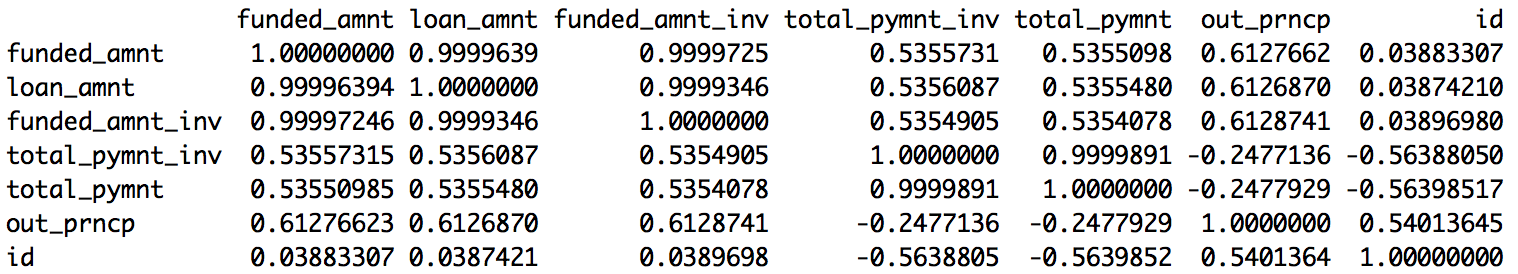
\includegraphics[scale=0.6]{img/redundantData.png}
	\caption{Macierz korelacji dla zmiennych o współczynniku korelacji przekraczającym 90\%.}
	\label{lc:redundantData}
\end{figure}

Na podstawie uzyskanych wyników (Rysunek \ref{lc:redundantData}) wyłączono z dalszej analizy następujące atrybuty:

\begin{itemize}
	\item \textit{funded\_amnt\_inv}, ze względu na korelację z \textit{funded\_amnt},
	\item \textit{total\_pymnt\_inv}, ze względu na korelację z \textit{total\_pymnt},
	\item \textit{funded\_amnt}, ze względu na korelację z \textit{loan\_amnt}.
\end{itemize}
Nie uwzględniano również zmiennej \textit{id}, ponieważ nie ma ona żadnego wpływu na zachowanie długu.

Następnie w oparciu udostępniony słownik danych \cite{LendingClub} wybrano atrybuty, które opisują pożyczkę oraz zdolność kredytową kredytobiorcy:

\begin{itemize}
	\item $loan\_amnt$ - kwota kredytu,
	\item $int\_rate$ - stopa procentowa,
	\item $term$ - okres spłaty kredytu,
	\item $emp\_length$ - okres zatrudnienia kredytobiorcy,
	\item $annual\_inc$ - roczny przychód kredytobiorcy,
	\item $delinq\_2yrs$ - liczba rat, które nie zostały spłacone w terminie w ciągu ostatnich 2 lat,
	\item $dti$ - stosunek zadłużenia do przychodu kredytobiorcy.
\end{itemize}

Ponadto utworzono zmienną $paid\_amount\_ratio$, określającą w jakim stopniu kredyt został już spłacony.

\subsubsection{Zależność pomiędzy wysokością pożyczki, a jej zachowaniem}

\begin{figure}[h] \centering %H if want to get it exaclty here
	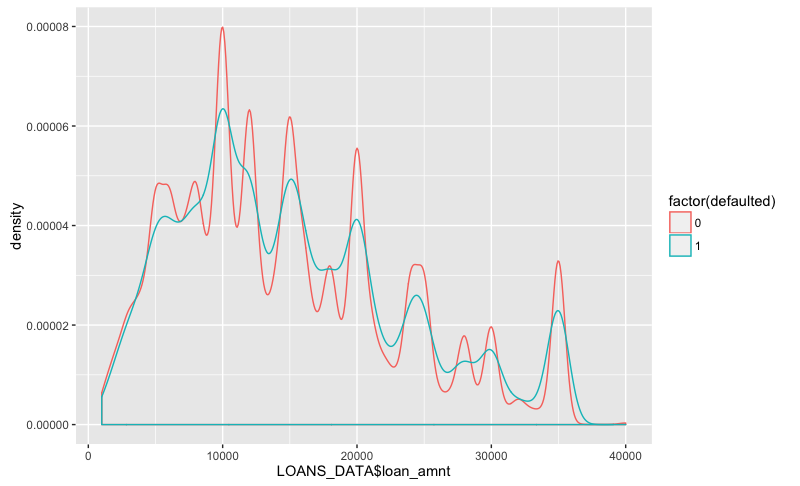
\includegraphics[scale=0.5]{img/amt_defaulted.png}
	\caption{Zależność pomiędzy wysokością pożyczki, a jej zachowaniem.}
	\label{lc:amt_defaulted}
\end{figure}

Wykres przedstawiający tę zależnosć (Rysunek \ref{lc:amt_defaulted}) charakteryzuje się dużą nieregularnością i nie można wydzielić przedziałów wysokości pożyczek, które jednoznacznie wskazywałyby na duże prawdopodobieństwo negatywnego lub pozytywnego zachowania kredytu.

\subsubsection{Zależność pomiędzy wysokością stóp procentowych, a zachowaniem pożyczki}

\begin{figure}[h] \centering %H if want to get it exaclty here
	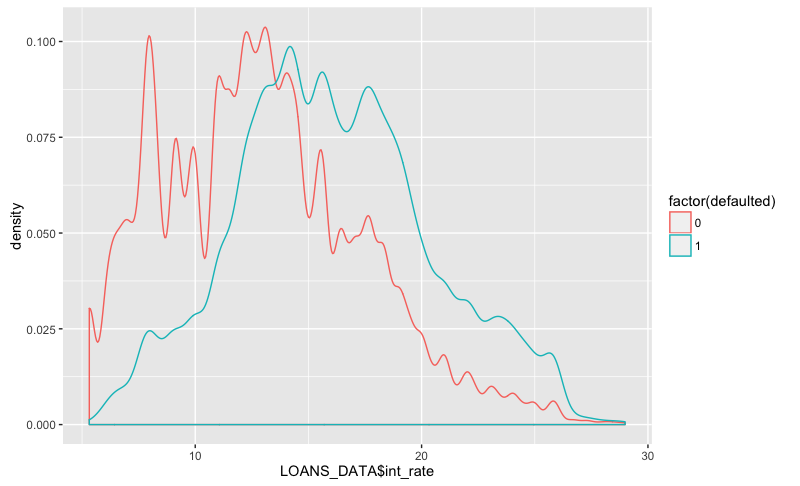
\includegraphics[scale=0.5]{img/int_defaulted.png}
	\caption{Zależność pomiędzy wysokością stóp procentowych, a zachowaniem pożyczki.}
	\label{lc:int_defaulted}
\end{figure}

W tym przypadku zależnosć jest zdecydowanie lepiej widoczna. Na podstawie wykresu (Rysunek \ref{lc:int_defaulted}) można stwierdzić, że prawdopodobieństwo negatywnego zachowania pożyczki znacząco wzrasta wraz z przekroczeniem progu 14\% stopy procentowej. Jest to uzasadnione tym, że wraz ze wzrostem ryzyka wzrasta oczekiwana przez inwestorów stopa zwrotu z inwestycji.

\subsubsection{Zależność pomiędzy okresem, na jaki zawarta jest pożyczka, a jej zachowaniem}

\begin{figure}[H] \centering %H if want to get it exaclty here
	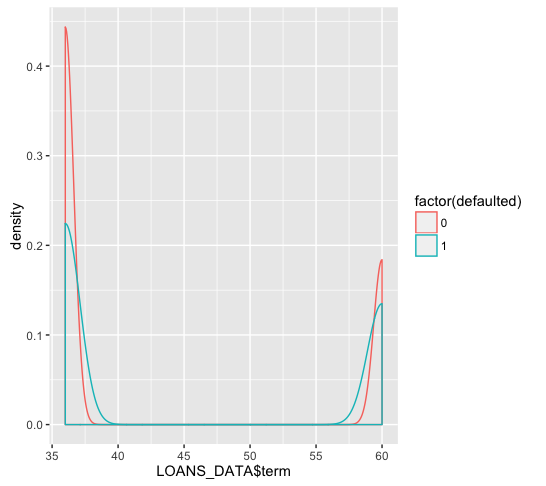
\includegraphics[scale=0.7]{img/term_defaulted.png}
	\caption{Zależność pomiędzy okresem, na jaki zawarta jest pożyczka, a jej zachowaniem.}
	\label{lc:term_defaulted}
\end{figure}

Na podstawie wykresu (Rysunek \ref{lc:term_defaulted}) można jednoznacznie stwierdzić, że dla pożyczek zawartych na krótszy okres czasu ryzyko jest zdecydowanie niższe, niż w przypadku kredytów 5-letnich.

\subsubsection{Zależność pomiędzy długością zatrudnienia kredytobiorcy, a zachowaniem pożyczki}

\begin{figure}[H] \centering %H if want to get it exaclty here
	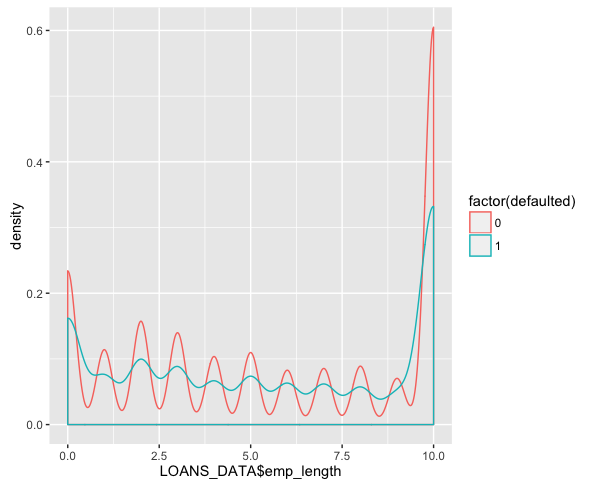
\includegraphics[scale=0.7]{img/emp_defaulted.png}
	\caption{Zależność pomiędzy długością zatrudnienia kredytobiorcy, a zachowaniem pożyczki.}
	\label{lc:emp_defaulted}
\end{figure}

Co zaskakujące, nie ma jednoznacznej zależności pomiędzy długością zatrudnienia kredytobiorcy, a zachowaniem zawieranej przez niego pożyczki (Rysunek \ref{lc:emp_defaulted}). Intuicja sugerowałaby, że wraz ze wzrostem stażu pracy, wzrośnie również stabilność ekonomiczna pożyczkobiorcy, a co za tym idzie spadnie ryzyko negatywnego zachowania pożyczki, jednak obie krzywe są nieregularne.

\subsubsection{Zależność pomiędzy rocznym dochodem kredytobiorcy, a zachowaniem pożyczki}

\begin{figure}[H] \centering %H if want to get it exaclty here
	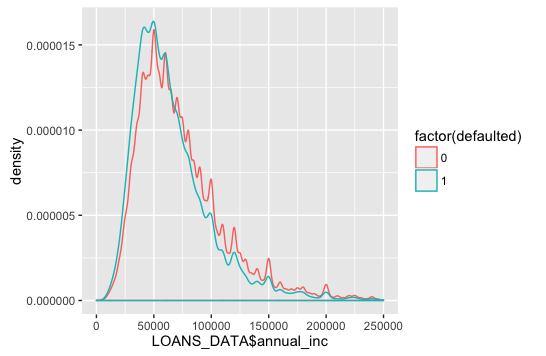
\includegraphics[scale=0.7]{img/inc_defaulted.png}
	\caption{Zależność pomiędzy długością zatrudnienia kredytobiorcy, a zachowaniem pożyczki.}
	\label{lc:inc_defaulted}
\end{figure}

Wysokość rocznego wynagrodzenia nie pozwala określenie prawdopodobnego zachowania pożyczki w zależności przyjętego przedziału dochodu - przebieg obu krzywych jest zbliżony (Rysunek \ref{lc:inc_defaulted}).

\subsubsection{Zależność pomiędzy liczbą spóźnionych rat, a zachowaniem pożyczki}

\begin{figure}[h] \centering %H if want to get it exaclty here
	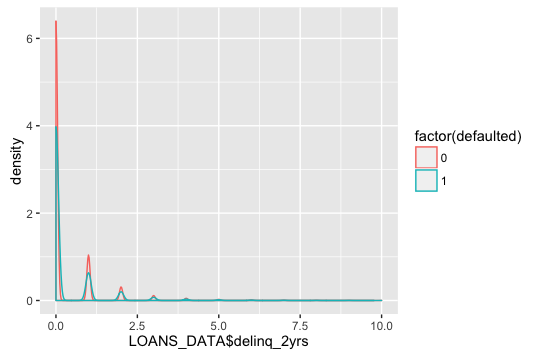
\includegraphics[scale=0.7]{img/delinq_defaulted.png}
	\caption{Zależność pomiędzy liczbą spóźnionych rat, a zachowaniem pożyczki.}
	\label{lc:delinq_defaulted}
\end{figure}

Wykres przedstawiający tę zależność (Rysunek \ref{lc:delinq_defaulted}), wskazuje większe prawdopodobieństwo pozytywnego zachowania pożyczki, jeśli kredytobiorca nigdy nie zalegał ze spłatą rat. W przypadku występowania spóźnionych rat obie krzywe przebiegają w zbliżony sposób.

\subsubsection{Zależność pomiędzy stosunkiem zadłużenia do dochodu kredytobiorcy, a zachowaniem pożyczki}

\begin{figure}[H] \centering %H if want to get it exaclty here
	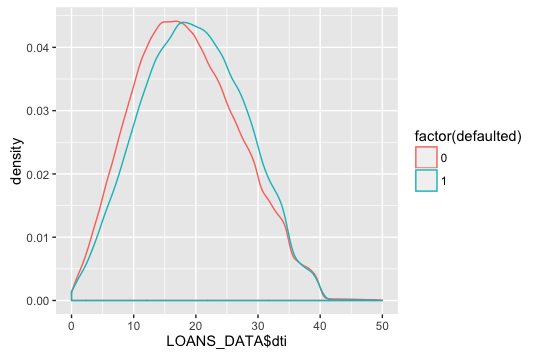
\includegraphics[scale=0.7]{img/dti_defaulted.png}
	\caption{Zależność pomiędzy stosunkiem zadłużenia do dochodu kredytobiorcy, a zachowaniem pożyczki.}
	\label{lc:dti_defaulted}
\end{figure}

Dla wartości zmiennej niższej niż 17\% isnieje większa szansa pozytywnego przebiegu inwestycji, w przypadku wyższych wartości nieznacznie wzrasta ryzyko negatywnego zachowania pożyczki, ale różnice w przebiegu krzywych są niewielkie (Rysunek \ref{lc:dti_defaulted}).

\subsubsection{Zależność pomiędzy stopniem spłaty pożyczki, a jej zachowaniem}

\begin{figure}[H] \centering %H if want to get it exaclty here
	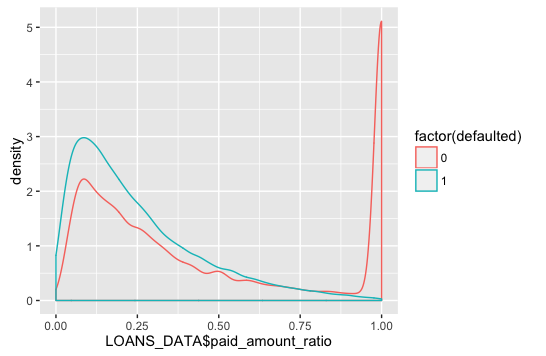
\includegraphics[scale=0.7]{img/paid_defaulted.png}
	\caption{Zależność pomiędzy stopniem spłaty pożyczki, a jej zachowaniem.}
	\label{lc:paid_defaulted}
\end{figure}

Na podstawie tego wykresu (Rysunek \ref{lc:paid_defaulted}), że pożyczki, dla których spłacono przynajmniej 80\% zadłużenia z dużą dozą prawdopodobieństwa zostaną spłacone do końca. Analogicznie dla pożyczek o stopniu spłacenia niższym niż 7\% wzrasta ryzyko niespłacenia pożyczki - oznaczałoby to osoby, które wzięły kredyt z góry zakładając, że nie będą go spłacać. Obie te informacje są cenną wskazówką dla inwestorów, a ponadto pozwalają na określenie przedziałów charakteryzujących się określonym zachowaniem pożyczki, co pozwala zakładać, że ta zmienna powinna zostać wykorzystana w procesie uczenia modelu predykcyjnego.

\subsubsection{Podsumowanie analizy zmiennych numerycznych}

Zmiennymi, od których wartości w największym stopniu zależy zachowanie pożyczki to \textbf{stopień spłaty pożyczki}, \textbf{stopy procentowe} oraz \textbf{okres, na jaki została zawarta pożyczka} - zostaną one wykorzystane przy uczeniu modelu predykcyjnego. Dużym zaskoczeniem jest brak wyraźnej zależności pomiędzy wysokością rocznego dochodu oraz stażem zatrudnienia, a potencjalnym zachowaniem pożyczki.